\documentclass{article}

\usepackage{tikz}
\usepackage{circuitikz}
\usepackage[utf8]{inputenc}
\usepackage[english,bulgarian]{babel}
\usepackage{graphicx}

\title{Приложение на математиката за моделиране на реални процеси. Моделиране на неврон.}
\author{Тонка Желева \and Васил Пашов}

\begin{document}

\maketitle
\newpage

\tableofcontents
\newpage
\title{TO DO}
\begin{enumerate}
    \item Науката за невроните и приложение
    \item Структура на неврона
        \begin{enumerate}
            \item Обобщено устройство на неврона
            \item Синапси
        \end{enumerate}
    \item Мембрана на неврона
    \item Аксонът на Ходжкинс-Хъксли
        \begin{enumerate}
            \item Изравняване на напрежението (Voltage Clamping)
        \end{enumerate}
    \item Извеждане на математическия модел и метод за решаване
    \item Програмна реализация на математическия модел и анимация
\end{enumerate}

\section{Науката за невроните и приложение}

Мозъкът, намиращ се в черепната кухина, е част от централната нервна ссистема. Той е основният орган, който обработва всички съзнателни и
несъзнателни стимули, чувства,  познания и памет. Също така е отговрен за контролирането на множество други органи. Основната градивна
единица на мозъка е неврона. Човешкия мозък съдържа около   неврона. Невронните клетки приемат, обработват и изпращат нервния импулс.
Животните реагират на външни въздействия, използвайки невроните.  Например при заплаха от изгаряне, рецепторите за топлина на сензорен
неврон осъществяват връзка със стимула и изпращат информация до интер-неврон в централната нервна система. От там мото-неврон изпраща
отговорът до скелетните мускули, които карат тялото да се отдръпне. В основата на извършването на този процес стои невротрансмисията, която
се извършва във всични неврони в човешкото тяло. Невроните пренасят тази информация чрез промени в електричесния потенциал на мембраната.

\section{Устройство на неврона}

аксон - най-издълженият израстък на неврона, чиято дължина може да надхвърли десетки хиляди пъти диаметъра на клетъчното тяло. Аксонът
извежда нервните импулси от клетъчното тяло, пренасяйки информация до друга клетка. Нервните импулси са еднопосочни в аксонът, но невронът
може да получи информация под формата на протеини които се придвижват от синапса до клетъчното ядро. Много неврони имат само един аксон, но
той се разклонява в много направления и така прави възможна комуникацията с много клетки.  нервен импулс – 

\section{Аксонът но Ходжкинс-Хъксли}
\subsection[Изравняване на напрежението]{Изравняване на напрежението\footnote{Voltages Clamping}}
    За да можем да изследваме напълно някое свойство на даден предмет, трябва да можем да го контролираме процесите, в които това свойство
    се проявява.  Един от най - важните ппроцеси за нас е процесът по обмяна на вещества.  Обмяната на вещества от своя страна, обаче влияе
    на напрежението в неврона, което от своя страна влияе на обмяната на веществана. Виждаме, че се получава цикличен процес, който се
    изследва много трудно. За наше щастие съществува начин, по който да фиксираме напрежението в неврона. Този метод са използвали Ходжкинс
    и Хъксли. Нека разгледаме следната схема.
    \begin{center}
        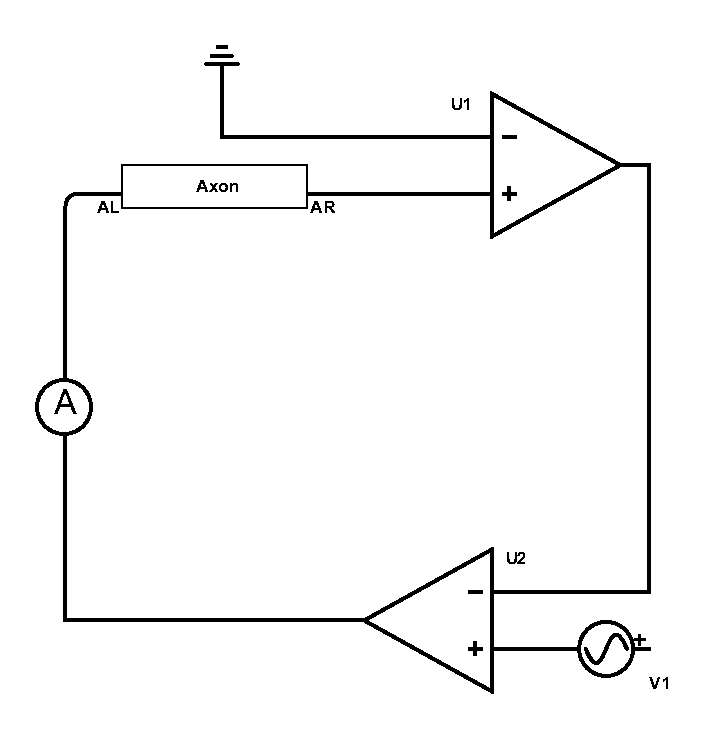
\includegraphics{./schemas/voltage-clamp.pdf}
    \end{center}
    През аксона е прокаран дълъг и тънък проводник, свързан с положителния вход на усилвател с коефициент 1. Отрицателният вход на усилвателя
    е заземен (или е свързан с течност като тази в която се намира неврона). По този начин усилвателя предава ток с напрежение $V_n$ равно на
    напрежението в самия неврон. Този ток се подава като отрицателен вход на друг усилвател с коефициент 1. На положителния вход на този
    усилвател се подава ток с напрежение двойно на желаното равновесно напрежение $V_d$. Този ток през амперметър и след това се подава в
    другия край на аксона. По точи начин ако $V_n > 2V_d$ в точката $AL$ напрежението ще бъде по - ниско от нормалното за акосна, за да се
    компенсира това положителните частици ще се насочат в тази посока, намаляки напрежението в аксона. Напрежението ще намалява клонейки към
    $V_n$ и когато стане равно на $V_n$ токът, излизащ от усилвател $U_2$ ще бъде с напрежение $U_d$, като така се получава равновесие в
    системата.

\end{document} 
